\documentclass[11pt,aspectratio=169]{beamer}

\usepackage[utf8]{inputenc}
\usepackage[T1]{fontenc}
\usepackage[french]{babel}
\usepackage{lmodern}
\usepackage{amsmath,amssymb}
\usepackage{booktabs}
\usepackage{graphicx}
\usepackage{tikz}
\usetikzlibrary{shadows}
\usepackage{pgfplots}
\pgfplotsset{compat=1.18}

\definecolor{templateblue}{RGB}{49,50,178}
\definecolor{deepblue}{RGB}{35,40,145}
\definecolor{softgray}{RGB}{245,246,248}
\definecolor{espritred}{RGB}{215,35,45}
\definecolor{femalepink}{RGB}{232,62,140}
\definecolor{maleblue}{RGB}{44,127,184}

\graphicspath{{../}{./}{graphes/}}

\setbeamertemplate{navigation symbols}{}
\setbeamercolor{normal text}{fg=black,bg=white}
\setbeamercolor{structure}{fg=templateblue}
\setbeamercolor{frametitle}{fg=white,bg=templateblue}
\setbeamercolor{block title}{fg=white,bg=deepblue}
\setbeamercolor{block body}{bg=softgray}
\setbeamerfont{frametitle}{series=\bfseries,size=\Large}
\setbeamerfont{normal text}{size=\large}
\setbeamerfont{block title}{series=\bfseries,size=\normalsize}
\setbeamerfont{block body}{size=\normalsize}

\setbeamertemplate{frametitle}{%
  \vspace{0.18cm}
  \begin{beamercolorbox}[wd=\paperwidth,ht=0.74cm,dp=0.18cm,leftskip=0.35cm]{frametitle}
    \usebeamerfont{frametitle}\insertframetitle
  \end{beamercolorbox}
}

\setbeamertemplate{footline}{%
  \leavevmode%
  \hbox{%
    \begin{beamercolorbox}[wd=.34\paperwidth,ht=2.5ex,dp=1ex,center]{frametitle}
      \scriptsize Groupe 2 DS (ESPRIT)
    \end{beamercolorbox}%
    \begin{beamercolorbox}[wd=.30\paperwidth,ht=2.5ex,dp=1ex,center]{frametitle}
      \scriptsize Actuariat Vie
    \end{beamercolorbox}%
    \begin{beamercolorbox}[wd=.23\paperwidth,ht=2.5ex,dp=1ex,center]{frametitle}
      \scriptsize A.U.2025--2026
    \end{beamercolorbox}%
    \begin{beamercolorbox}[wd=.13\paperwidth,ht=2.5ex,dp=1ex,center]{frametitle}
      \scriptsize \insertframenumber/15
    \end{beamercolorbox}%
  }%
}

\title{Prix de rentes viagères genrés et unisexe}
\subtitle{Projet Actuariat Vie -- Sujet 3}
\author{Groupe 2 DS}
\date{A.U.2025--2026}

\begin{document}

\begin{frame}[plain]
  \vspace{0.35cm}
  \begin{columns}[T,totalwidth=0.90\paperwidth]
    \begin{column}{0.50\textwidth}
      
\includegraphics[height=1.25cm,trim=16 75 16 75,clip]{logo_esprit.png}
    \end{column}
    \begin{column}{0.50\textwidth}
      \raggedleft
\includegraphics[height=1.25cm,trim=13 11 14 9,clip]{logo_ira.png}
    \end{column}
  \end{columns}

  \vspace{1.25cm}
  \begin{center}
    \begin{tikzpicture}
      \node[
        fill=templateblue,
        text=white,
        rounded corners=3pt,
        drop shadow,
        inner xsep=0.55cm,
        inner ysep=0.24cm,
        minimum width=0.88\paperwidth
      ] {\Large\bfseries Prix de rentes viagères genrés et unisexe};
    \end{tikzpicture}

    \vspace{0.55cm}
    {\large Projet Actuariat Vie -- Sujet 3}

    \vspace{0.25cm}
    {\small Groupe 2 DS : Amine Manai, Maha Aloui, Nassir Bouzaiene, Yasmine Attyaoui}

    \vspace{0.32cm}
    {\normalsize Enseignants : Anis Matoussi et Wissal Sabbagh}

    \vspace{0.25cm}
    {\normalsize A.U.2025--2026}

    \vspace{0.18cm}
    {\footnotesize Lien vidéo de présentation : \href{https://1drv.ms/v/c/d2f2bab425a55620/IQClckgZFiD3RY0VaD47N5IjAU5EfMcGudapIm3BismdfnE?e=QHEJKQ}{Cliquez ici pour accéder à la vidéo}}
  \end{center}
\end{frame}

\begin{frame}{Organisation du groupe}
  \begin{block}{Déclaration d'utilisation de l'IA générative}
    Une IA générative a été utilisée pour aider à structurer le rapport, la présentation et certaines reformulations. Les méthodes, calculs et interprétations suivent le cours ActVie\_M1\_2025-26 et le sujet 3.
  \end{block}

  \vspace{0.12cm}
  \begin{center}
  \begin{tabular}{p{3.1cm}p{8.9cm}}
    \toprule
    Membre & Questions principales traitées \\
    \midrule
    Amine Manai & Q1--Q2 : données HMD, estimation MV et intervalles de confiance. \\
    Maha Aloui & Q3--Q4 : extraction de cohorte et projection centrale avec \texttt{forecast}. \\
    Nassir Bouzaiene & Q5--Q6 : log-taux depuis 2005 et VAP par genre. \\
    Yasmine Attyaoui & Q7--Q8 : prime unisexe, méthode 60/40 et transfert de risque. \\
    \bottomrule
  \end{tabular}
  \end{center}
\end{frame}

\begin{frame}{Q1 -- Données HMD}
  \begin{block}{Pays et séries}
    Les assurés sont anglais : on retient la base HMD \texttt{GBRTENW}, c'est-à-dire Angleterre et Pays de Galles.
  \end{block}

  \vspace{0.18cm}
  \begin{itemize}
    \item Données téléchargées depuis la Human Mortality Database.
    \item Séries utilisées : femmes, hommes et population totale.
    \item Conversion en objet \texttt{StMoMoData} pour appliquer le package \texttt{StMoMo}.
    \item Cohorte étudiée : assurés nés en 1955, contrat entre 2015 et 2045.
  \end{itemize}

  \vspace{0.12cm}
  \begin{block}{Commentaire}
    La base fournit les âges, les années, les expositions et les taux observés. On peut donc séparer les calculs par genre puis comparer avec la série totale.
  \end{block}
\end{frame}

\begin{frame}{Q2 -- Estimation par maximum de vraisemblance}
  \begin{columns}[T,totalwidth=\textwidth]
    \begin{column}{0.40\textwidth}
      {\scriptsize
      \begin{block}{Idée statistique}
        Sous l'hypothèse \(D_{x,t} \sim \mathcal{P}(E_{x,t}\mu_{x,t})\), l'estimateur MV est :
        \[
          \widehat{\mu}_{x,t}=\frac{D_{x,t}}{E_{x,t}}.
        \]
      \end{block}

      \begin{block}{Commentaire}
        IC à 95\% en pointillés. Les taux masculins sont globalement plus élevés.
      \end{block}
      }
    \end{column}
    \begin{column}{0.58\textwidth}
      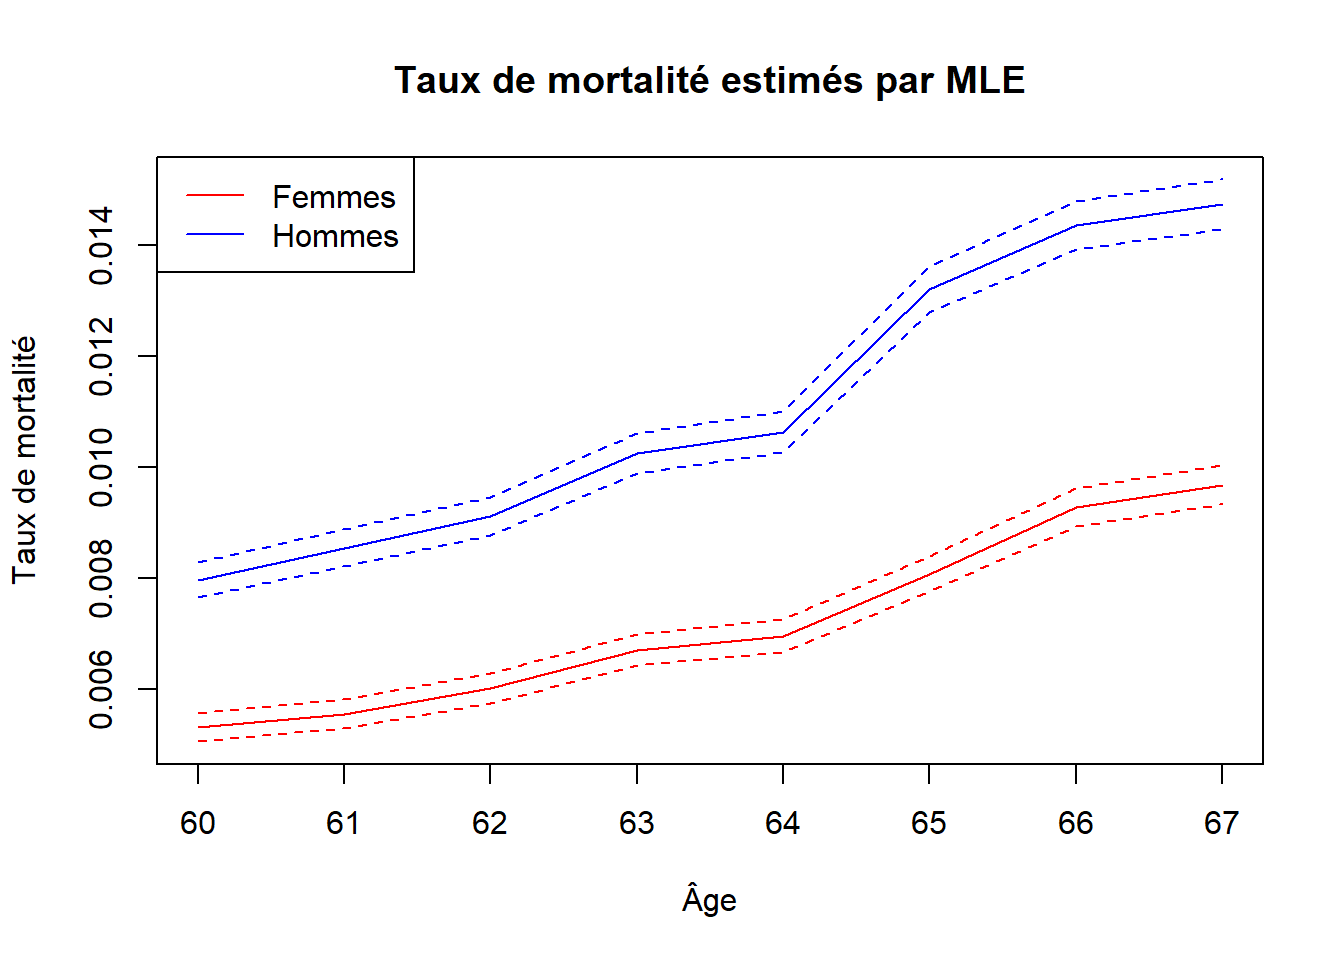
\includegraphics[width=0.96\textwidth]{rapport_graphe_01.png}
    \end{column}
  \end{columns}
\end{frame}

\begin{frame}{Q3 -- Lecture cohorte avec extractCohort}
  \begin{columns}[T,totalwidth=\textwidth]
    \begin{column}{0.36\textwidth}
      {\scriptsize
      \begin{block}{Principe}
        \texttt{extractCohort} extrait la diagonale âge--année correspondant à une même génération.
      \end{block}

      \begin{block}{Commentaire}
        Pour la cohorte 1955, \(t=x+1955\). La lecture est longitudinale : elle suit les mêmes assurés pendant le contrat.
      \end{block}
      }
    \end{column}
    \begin{column}{0.62\textwidth}
      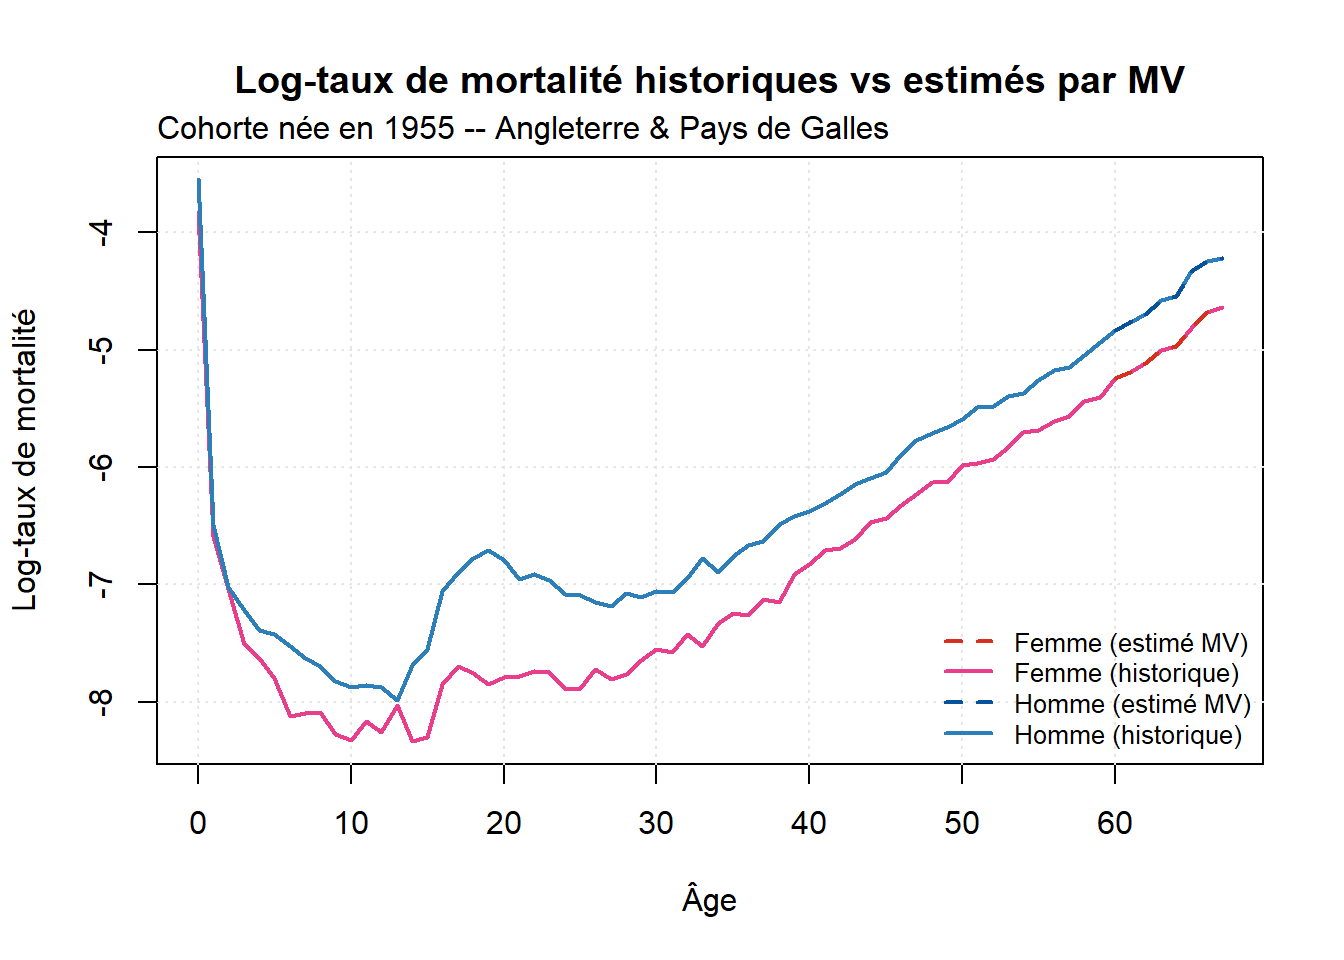
\includegraphics[width=0.98\textwidth]{rapport_graphe_02.png}
    \end{column}
  \end{columns}
\end{frame}

\begin{frame}{Q4 -- Projection centrale à 25 ans}
  \begin{columns}[T,totalwidth=\textwidth]
    \begin{column}{0.30\textwidth}
      {\scriptsize
      \[
        \log(\mu_{x,t}) = a_x + b_x k_t + \varepsilon_{x,t}
      \]
      \begin{block}{Réponse}
        La projection centrale est la trajectoire moyenne prévue par \texttt{forecast}.
      \end{block}
      \begin{itemize}
        \item La courbe noire prolonge \(k_t\) sur 25 ans.
        \item Les bandes grises donnent l'incertitude autour de cette moyenne.
        \item Quand \(k_t\) baisse, les taux de mortalité projetés diminuent.
      \end{itemize}
      }
    \end{column}
    \begin{column}{0.69\textwidth}
      \vspace{0.10cm}
      \begin{center}
        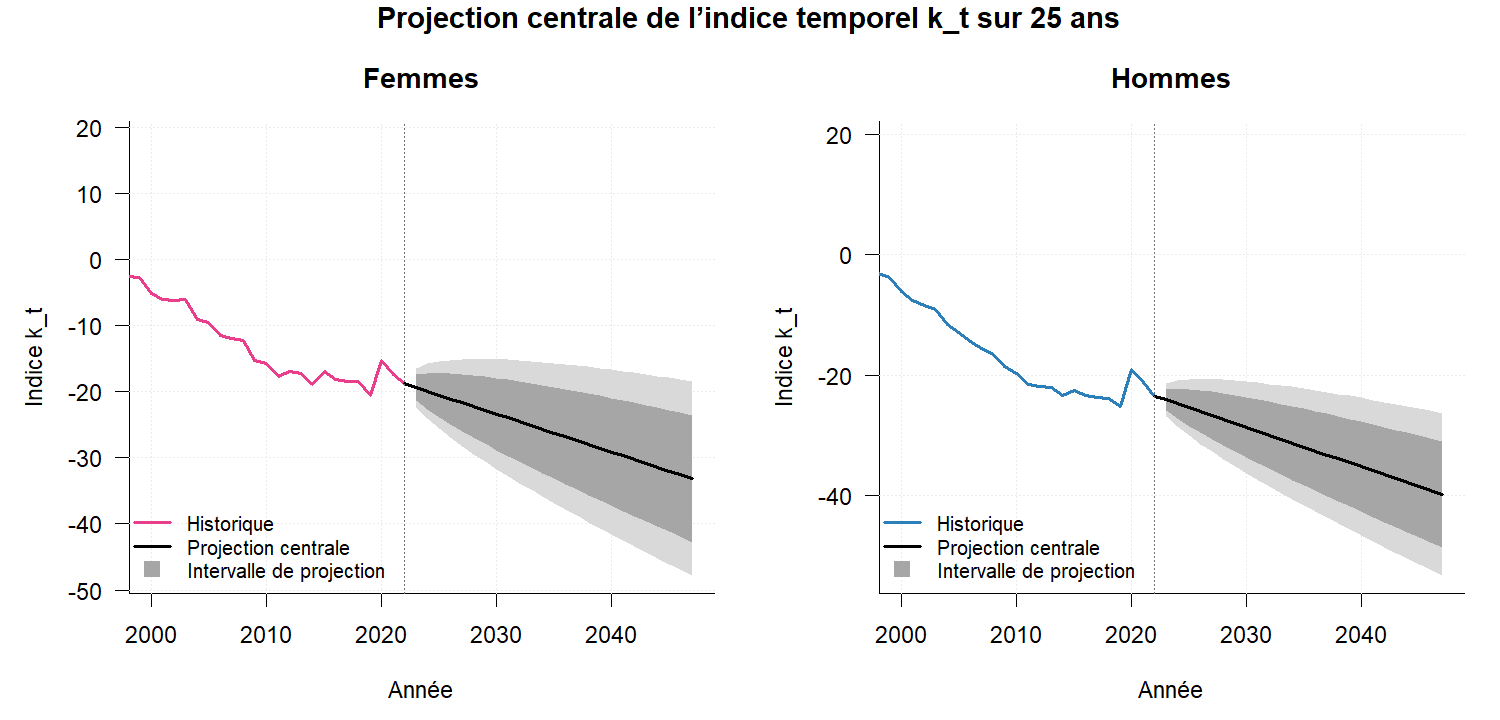
\includegraphics[width=1.06\textwidth]{projection_kt_25ans.png}
      \end{center}
    \end{column}
  \end{columns}
\end{frame}

\begin{frame}{Q5 -- Log-taux historiques depuis 2005}
  \begin{columns}[T,totalwidth=\textwidth]
    \begin{column}{0.38\textwidth}
      \begin{block}{Pourquoi 2005 ?}
        La cohorte née en 1955 a 50 ans en 2005. On observe donc sa trajectoire avant l'entrée dans le contrat en 2015.
      \end{block}

      \begin{block}{Commentaire}
        Les log-taux augmentent avec l'âge. Les hommes restent au-dessus des femmes, ce qui traduit une mortalité masculine plus élevée.
      \end{block}
    \end{column}
    \begin{column}{0.60\textwidth}
      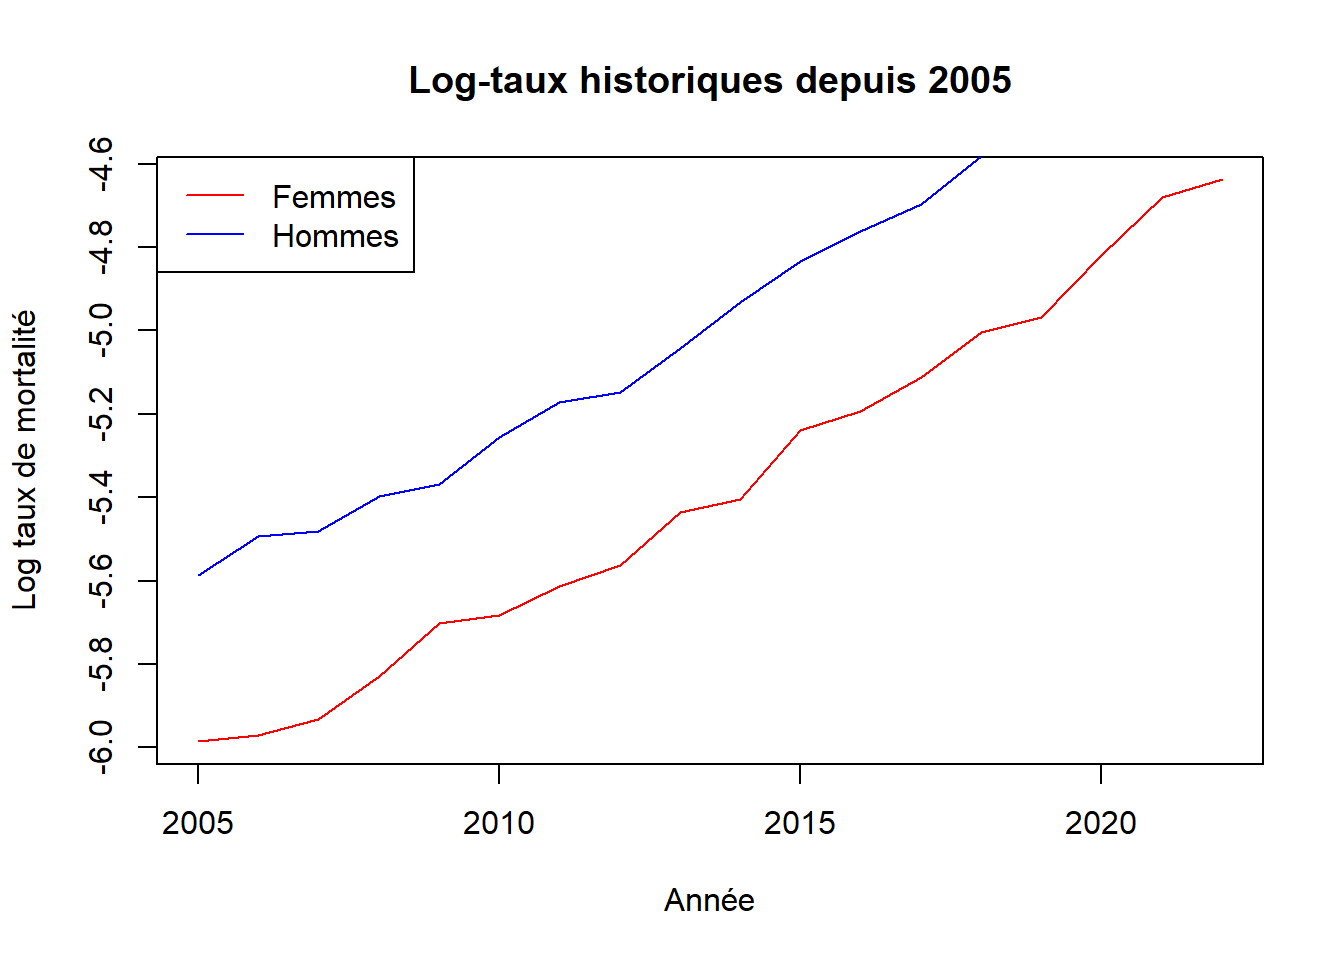
\includegraphics[width=\textwidth]{rapport_graphe_05.png}
    \end{column}
  \end{columns}
\end{frame}

\begin{frame}{Q6 -- Valeur actuelle probable par genre}
  \begin{block}{Formule de la rente temporaire}
    Pour une rente à termes anticipés :
    \[
      VAP=\sum_{k=0}^{n-1} v^k\,{}_kp_x,
      \qquad v=\frac{1}{1+i}.
    \]
  \end{block}

  \vspace{0.18cm}
  \begin{columns}[T,totalwidth=\textwidth]
    \begin{column}{0.50\textwidth}
      \begin{center}
      \begin{tabular}{lc}
        \toprule
        Série & VAP estimée \\
        \midrule
        Femmes & 19.49538 \\
        Hommes & 18.16818 \\
        \bottomrule
      \end{tabular}
      \end{center}
    \end{column}

    \begin{column}{0.46\textwidth}
      \begin{block}{Commentaire}
        On observe que la VAP féminine est plus élevée. Cela traduit une mortalité plus faible et donc une durée probable de paiement plus longue.
      \end{block}
    \end{column}
  \end{columns}
\end{frame}

\begin{frame}{Q7 -- Prime unisexe avec la série Total}
  \begin{block}{Principe}
    En tarification unisexe, l'assureur ne différencie pas le prix selon le genre. On peut donc utiliser la série \texttt{total} de HMD.
  \end{block}

  \vspace{0.12cm}
  \begin{center}
  \begin{tabular}{lc}
    \toprule
    Méthode & Prime pure \\
    \midrule
    Femmes & 19.49538 \\
    Hommes & 18.16818 \\
    Unisexe population totale & 18.81099 \\
    \bottomrule
  \end{tabular}
  \end{center}

  \vspace{0.08cm}
  \begin{block}{Commentaire}
    La série \texttt{total} donne une prime unisexe simple, mais elle ne reflète pas forcément la structure réelle du portefeuille.
  \end{block}
\end{frame}

\begin{frame}{Q8 -- Méthode unisexe adaptée au portefeuille}
  \begin{block}{Portefeuille observé}
    Le portefeuille contient 60\% de femmes et 40\% d'hommes. Une prime unisexe adaptée au portefeuille est :
    \[
      \Pi_{60/40}=0.60\,VAP_F+0.40\,VAP_H.
    \]
  \end{block}

  \vspace{0.12cm}
  \begin{center}
  \begin{tabular}{lc}
    \toprule
    Méthode & Prime pure \\
    \midrule
    Unisexe population totale & 18.81099 \\
    Unisexe portefeuille 60/40 & 18.96450 \\
    \bottomrule
  \end{tabular}
  \end{center}

  \vspace{0.08cm}
  \begin{block}{Commentaire}
    La prime 60/40 tient compte de la composition observée. Elle est donc plus adaptée au portefeuille étudié que la série totale brute.
  \end{block}
\end{frame}

\begin{frame}{Synthèse numérique}
  \vspace{0.25cm}
  \begin{center}
  \renewcommand{\arraystretch}{1.35}
  \begin{tabular}{lcc}
    \toprule
    Méthode & Données utilisées & VAP / prime pure \\
    \midrule
    Femmes & Cohorte 1955 femmes & 19.49538 \\
    Hommes & Cohorte 1955 hommes & 18.16818 \\
    Unisexe série Total HMD & Population globale & 18.81099 \\
    Unisexe portefeuille 60/40 & 60\% femmes, 40\% hommes & 18.96450 \\
    \bottomrule
  \end{tabular}
  \end{center}

  \vspace{0.45cm}
  \begin{block}{Lecture}
    La VAP féminine est la plus élevée, car la mortalité féminine est plus faible. La prime 60/40 est supérieure à la prime issue de la série Total HMD, car le portefeuille contient davantage de femmes.
  \end{block}
\end{frame}

\begin{frame}{Commentaire actuariel}
  \begin{itemize}
    \item La mortalité féminine plus faible augmente la durée probable de paiement.
    \item La prime masculine est plus faible en tarification genrée, car les paiements attendus sont moins longs.
    \item Une prime unisexe crée un transfert de risque : les hommes paient au-dessus de leur coût propre, les femmes en dessous.
    \item La méthode 60/40 est plus juste pour ce portefeuille que la série \texttt{total}, car elle utilise la structure réelle des assurés.
  \end{itemize}
\end{frame}

\begin{frame}{Limites et approfondissements}
  \begin{block}{Limites principales}
    Les résultats dépendent du taux d'intérêt, de la période de calibration du modèle et de la stabilité future de la mortalité.
  \end{block}

  \vspace{0.12cm}
  \begin{itemize}
    \item Tester d'autres taux d'actualisation pour mesurer la sensibilité de la VAP.
    \item Comparer Lee-Carter avec d'autres modèles de mortalité de \texttt{StMoMo}.
    \item Étudier l'effet d'une composition de portefeuille différente de 60/40.
  \end{itemize}
\end{frame}

\begin{frame}{Conclusion}
  \begin{itemize}
    \item Le projet passe d'une mortalité observée à une mortalité projetée.
    \item Les probabilités de survie déduites des taux projetés déterminent directement la VAP.
    \item Les femmes ont une VAP plus élevée, ce qui traduit une longévité attendue plus forte.
    \item La prime \texttt{total} est simple ; la prime 60/40 reflète mieux le portefeuille.
    \item Le transfert de risque vient de la mutualisation imposée par la tarification unisexe.
  \end{itemize}
\end{frame}

\begin{frame}{Références}
  \begin{itemize}
    \item Cours ActVie\_M1\_2025-26.
    \item Human Mortality Database, données Angleterre et Pays de Galles.
    \item Villegas, Kaishev et Millossovich, \emph{StMoMo: An R Package for Stochastic Mortality Modeling}.
    \item Brouhns, Denuit et Vermunt, modèle de Poisson log-bilinéaire pour la mortalité.
    \item Lee et Carter, modélisation et prévision de la mortalité.
  \end{itemize}
\end{frame}

\end{document}
